\begin{frame}{VIBeS - ESA ARTES  6A.054}

  This thesis is inspired by the European Space Agency VIBeS (\emph{VI}rtualized
  NFs for \emph{B}roadband \emph{S}atellite networks) project

  \vfill{}

  The goal is to exploit NFV and TCP/IP stack optimizations to enhance
  communication paths that involve a \textbf{satellite} link

  \vfill{}

  Redesign and orchestrate a Performance Enhancement Proxy (\textbf{PEP}) as
  virtualized functions

  \vfill{}

  \begin{figure}
    \centering
    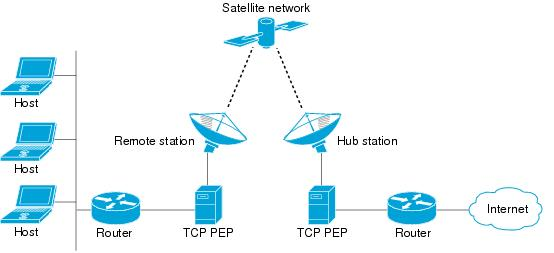
\includegraphics[scale=0.35]{pep}
  \end{figure}

\end{frame}